\documentclass{article}
\usepackage[utf8]{inputenc}

\title{TT3010 - Audio technology and room acoustics. \newline Exercise 5 - Microphones and loudspeakers \newline Solutions}


\author{Jan Arne Bosnes}
\date{\today}

\usepackage{natbib}
\usepackage{graphicx}
\usepackage{multicol}
\usepackage{gensymb}
\usepackage{float}
\usepackage{amsmath}


\begin{document}

\maketitle




\section{}

As we know from reading chap. 20.4 on microphone sensitivity, we know that the voltage sensitivity, $S_v$ (given in dB) is related to open circuit voltage $V$ and pressure $p$ as:

\begin{equation*}
    S_v = 20 \log{\frac{v}{p}} {\rm\ \  dB\ re.\ 1 V/Pa}
\end{equation*}

We can then rearrange the terms to express voltage in terms of voltage sensitivity and pressure.

\begin{equation*}
    \log{\frac{v}{p}}=\frac{S_v}{20}
\end{equation*}

\begin{equation}
    v=p\cdot 10^{\frac{S_v}{20}}
\label{eq:v}
\end{equation}

If $v_A$ and $S_{v,A}$ represent the voltage output and sensitivity of the first microphone, while $v_B$ and $S_{v,B}$ represent the voltage output and sensitivity of the second microphone, we can divide $v_A$ by $v_B$ to find the ratio between them, and $p$ disappears:

\begin{equation*}
    \frac{v_A}{v_B}=\frac{10^{\frac{S_{v,A}}{20}}}{10^{\frac{S_{v,B}}{20}}}
\end{equation*}

\begin{equation*}
    \frac{v_A}{v_B}=10^{\frac{S_{v,A}-S_{v,B}}{20}} = 10^{\frac{-60-(-66)}{20}} \approx 2
\end{equation*}

\section{}

The output voltage of the microphone can be determined by using the formula for the sensitivity, rewritten as in Eq. (\ref{eq:v})

%\begin{equation*}
%    \frac{S_V(dBV)}{20} = \log{\frac{V}{p}}
%\end{equation*}

%\begin{equation*}
%    \frac{V}{p} = 10^{\frac{S_V(dBV)}{20}}
%\end{equation*}

\begin{equation*}
    v = p \cdot 10^{\frac{S_V}{20}} = 1 \cdot 10^{-60/20} \ {\rm V} = 10^{-3} \ {\rm V} = 1 \ {\rm mV}
\end{equation*}

%\textbf{Remember} we have to check that the open-circuit voltage sensitivity is per voltage. To check for this we do the following.

%\begin{equation*}
%    V=(10^{-3} V) (1000 \frac{mV}{V}) = 1 \ mV
%\end{equation*}

%Therefore the output voltage of the microphone is 1 mV.

To find the sound pressure $p$, we use

\begin{equation*}
    L_p=20 \log{\frac{p}{p_0}}
\end{equation*}
where $p_0$ is reference sound pressure for the sound pressure level and is given as $p_0 = 20 \mu \ {\rm Pa}$. The sound pressure level for a sound pressure of 1 Pa, will then be, 
\begin{equation*}
    L_p=20\log{\frac{1 {\rm Pa}}{20 \cdot 10^{-6}\ {\rm Pa}}} = 94 \ {\rm dB}
\end{equation*}

Therefore, the sound pressure level for a sound pressure of 1 Pa is 94 dB.

\section{}

We can find from Rossing chapter 25.3 that the angle of the sound image, $\theta_l$, has the following relation to the angle from the median plane that the loudspeakers are placed at, $\theta_A$, and the pressure from the left speaker, $p_L$, and the right speaker $p_R$.

\begin{equation}
    \frac{\sin(\theta_l)}{sin(\theta_A)} = \frac{p_L - p_R}{p_L+p_R}
\end{equation}

If the loudspeaker on the left has twice the amplitude than the one on the right, we can assume that $p_L=2p_R$. By rewriting the formula and inserting this relation, we get the following:

\begin{equation}
    \sin(\theta_l)=\frac{p_L - p_R}{p_L+p_R} \cdot \sin(\theta_A) = \frac{2p_R - p_R}{2p_R+p_R} \cdot \sin(30) = \frac{1}{3} \cdot \frac{1}{2} \rightarrow \theta_l \approx 10 \degree
\end{equation}

As shown, the image will resemble figure \ref{fig:img} where the image is shifted 10 degrees to the left.

\begin{figure}[H]
    \centering
    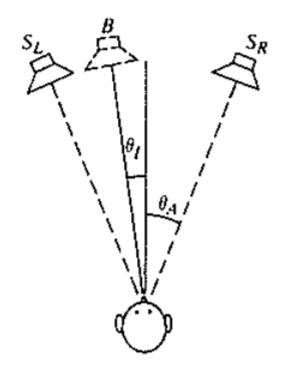
\includegraphics[scale=1.5]{figures/oving2_2.png}
    \caption{The changed sound image when the signal strength is increased in the left speaker.}
    \label{fig:img}
\end{figure}

\end{document}

